
\section{The Urban Observatory: CityScope Kendall Square}

 {
  One of the first instances of CityScope was the `Urban Observatory' \cite{Hadhrawi2016}. It was firstly constructed as part of a City Science Workshop by MIT students in 2013, to communicate and visualize corresponding spatial layers. The Urban Observatory was a dynamic visualization tool, designed to replace static models of cities, and provide expert and non-experts with a decision-support system. It employed a set of pre-defined spatial analytics layers, an array of a video projection mapping, and 3D physical models. The Urban Observatory was used as a `sandbox' platform and research context, on which observations and developed proposals for new urban-design for a site in Cambridge, MA were displayed.

  \begin{figure}[h]
      \begin{center}
          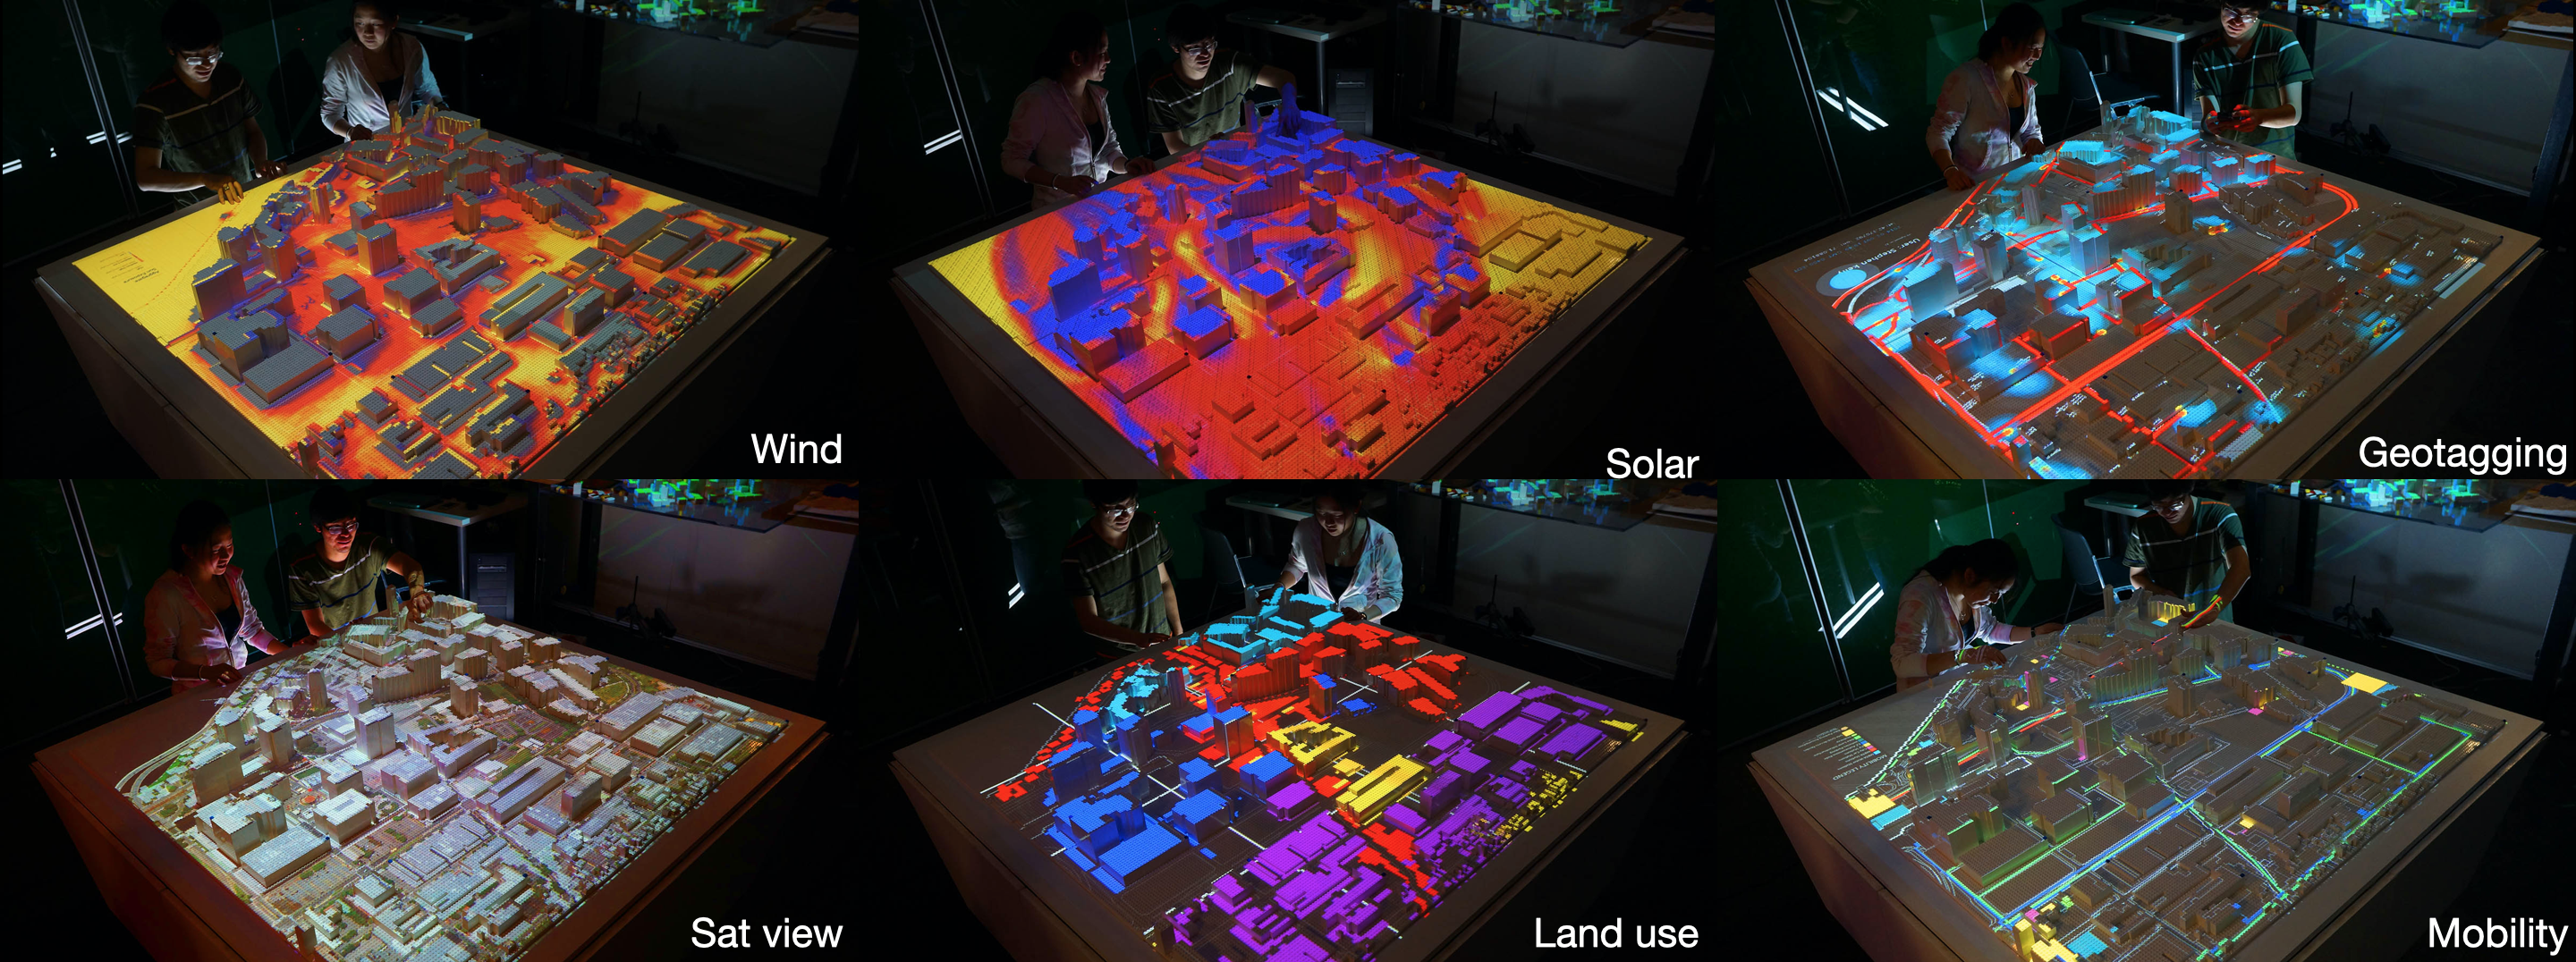
\includegraphics[width=1\textwidth]{chapters/insight/observatory/figures/urban_obs.png}
      \end{center}
      \caption{The Urban Observatory. Different layers of precomputed urban analysis projected onto a 3D model of the Kendall Sq. area in Cambridge, MA.}
      \label{fig:urban_obs}
  \end{figure}

  \subsection{System Design}
  {
      The Urban Observatory comprised of physical components, computer hardware, and custom display software, detailed bellow.

      \subsubsection{Computation}{\label{sec:computational-models}}
      {
          The Urban Observatory was design as an open canvas for displaying different layers of data, such as the formal properties of building designs, land-use, human activity and mobility, vehicular circulation, flows of energy, wind and solar exposure, and more (see Figure \eqref{fig:urban_obs}). These layers were pre-rendered in advance, since the platform was not set to perform spatial analytics or data acquisition in real-time\footnote{In later versions of CityScope, data for similar layers was fetched in real-time, and was rendered dynamically to reflect updated insights or user-interaction. See Chapter \eqref{ch:transformation}}. As part of the students' workshop, architectural, urban-planning, traffic-simulation, and visualization tools were all used to produce these data layers. The projection were projected and aligned to the 3D model using a Processing sketch \cite{reas2007processing}.
      }

      \subsubsection{Hardware}
      {
          The system contained two main elements: (i) a 3D urban model, made out of white LEGO bricks, and (ii) an array of overhang projectors. The physical model was of size $1.7m^2$, which represent a $1km^2$ area of Kendall Square, roughly as the scale of $4m$ for each LEGO stud. For projection, six video projectors were used: two to project the ground and roof planes of a physical model, and one projector for each of the four vertical surface orientations (north, south, east, and west), creating the illusion of 360$^{\circ}$ projection.
      }
  }

  \subsection{Usage}
  {
      The `Urban Observatory' was developed and situated in an active demonstration space at the MIT Media Lab building. Between '13-'16, hundreds of visitors, researchers, and students interacted with the installation; In 2015-2016, the platform was repurposed to support \textit{MAS.S65: The City Science Workshop}, an MIT course that was focused on prototyping new ways to collect and represent urban insights and spatial data. These insights were broad, and ranged from analyzing crime and energy, to vegetation and thermal comfort. Later that year, the 3D models was again repurposed to set as the base line for the CityScope Volpe project (see Section \eqref{sec:cityscope_volpe}).
  }

  \subsection{Discussion}{\label{subsec:observatory_discussion}}

  {
      The Urban Observatory was an early CityScope prototype, which projected pre-defined data layers and urban observations onto a tangible interface. Despite its simplicity, this prototype proven the advantage of merging spatial data and tangible interfaces, as a means to create a new `common ground' for urban discourse. This work also hinted to several features of future CityScope, such as: (i) A Data Warehouse that would store urban data, and spatial analytics algorithms (later to become cityIO, see Section \eqref{subsec:csarch-cityio}); (ii) User Interface, to provide a flexible and intuitive interaction for exploring different urban scenarios (such as CityScope TUI, see Section \eqref{subsec:mocho-volpe}); (iii) Interactive visualizations, to provide dynamic feedback to the users' design iteration (later to become CityScopeJS, see Section \eqref{sec:cityscope_architecture}). Arguably, the Urban Observatory's greatest contribution to the future of CityScope, was the idea of an open-ended urban `sandbox', on which new scenarios could be tested, and user contributions, feedback, and insights, would be collected.
      \newline
      As shown in the following work, later CityScope projects centered around behavioral, social, and economic insights, in order to look beyond the formal and physical aspects of the city.
  }
 }